\documentclass[10pt, a4paper]{amsart}
% \documentclass[10pt,showpacs,preprintnumbers,footinbib,amsmath,amssymb,aps,prl,twocolumn,groupedaddress,superscriptaddress,showkeys]{revtex4-1}
\usepackage[]{graphicx}
\usepackage[]{hyperref}
\usepackage[]{physics}
\usepackage[]{listings}
\usepackage[T1]{fontenc}
\usepackage{color}
\usepackage[ruled,vlined]{algorithm2e}

\usepackage{amsmath, amsfonts, amssymb}
\usepackage{listings}
\usepackage[]{subcaption}

% Definition of code and how the code should look.
\usepackage{xcolor}
\definecolor{codegreen}{rgb}{0,0.6,0}
\definecolor{codegray}{rgb}{0.5,0.5,0.5}
\definecolor{codepurple}{rgb}{0.58,0,0.82}
\definecolor{backcolour}{rgb}{0.95,0.95,0.92}
\definecolor{mygreen}{rgb}{0,0.6,0}
\definecolor{mymauve}{rgb}{0.58,0,0.82}


\lstdefinestyle{python3}{
    backgroundcolor=\color{backcolour},
    commentstyle=\color{codegreen},
    keywordstyle=\color{magenta},
    numberstyle=\tiny\color{codegray},
    stringstyle=\color{codepurple},
    basicstyle=\ttfamily\footnotesize,
    breakatwhitespace=false,
    breaklines=true,
    captionpos=b,
    keepspaces=true,
    numbers=left,
    numbersep=5pt,
    showspaces=false,
    showstringspaces=false,
    showtabs=false,
    tabsize=2
}
% End def.



\lstset{ %
  backgroundcolor=\color{white},   % choose the background color; you must add \usepackage{color} or \usepackage{xcolor}
  basicstyle=\footnotesize,        % the size of the fonts that are used for the code
  breakatwhitespace=false,         % sets if automatic breaks should only happen at whitespace
  breaklines=true,                 % sets automatic line breaking
  captionpos=b,                    % sets the caption-position to bottom
  commentstyle=\color{mygreen},    % comment style
  deletekeywords={...},            % if you want to delete keywords from the given language
  escapeinside={\%*}{*)},          % if you want to add LaTeX within your code
  extendedchars=true,              % lets you use non-ASCII characters; for 8-bits encodings only, does not work with UTF-8
  frame=single,	                   % adds a frame around the code
  keepspaces=true,                 % keeps spaces in text, useful for keeping indentation of code (possibly needs columns=flexible)
  keywordstyle=\color{blue},       % keyword style
  language=python,                    % the language of the code
  style = python3,
  otherkeywords={*,...},           % if you want to add more keywords to the set
  rulecolor=\color{black},         % if not set, the frame-color may be changed on line-breaks within not-black text (e.g. comments (green here))
  showspaces=false,                % show spaces everywhere adding particular underscores; it overrides 'showstringspaces'
  showstringspaces=false,          % underline spaces within strings only
  showtabs=false,                  % show tabs within strings adding particular underscores
  stepnumber=2,                    % the step between two line-numbers. If it's 1, each line will be numbered
  stringstyle=\color{mymauve},     % string literal style
  tabsize=2,	                     % sets default tabsize to 2 spaces
}

\title[Problem set 1]{Problem set 1: GEO2300: \\
\normalsize{Due: 16 Sept. 2020} \\
  \hrulefill\small{ GEO2300: Fysiske prosesser i geofag }\hrulefill}

\author[Sundberg]{Sigurd Sandvoll Sundberg}
\date{\today}

\begin{document}

\begin{titlepage}
\maketitle
\tableofcontents
\end{titlepage}

\section{Problem 1: Matricies}
In this section we will study the properties of matricies. How they are used to solve a system of linear equations, inverting matricies and finding eiegenvalues and eigenvectors, and lastly expressing matricies as a sum of eigenvectors and exponentials with corresponding eigenvalues. 

First we will look at solving the following system of linear equations as a matrix equation
\begin{equation}\label{eq:sys_linear}
\begin{split}
	x + 2y + z &= -1\\
	2x - y + 3z &= -5 \\
	-x + 3y- z &= 6
\end{split}
\end{equation}
We can rewrite Eq: \ref{eq:sys_linear} on the form $\mathbf{A}\vec{x} = \vec{b}$
\begin{equation}
	\begin{bmatrix}
		1 & 2 & 1 & -1\\
		2 & -1 & 3 & -5 \\
		-1 & 3 & -1 & 6
	\end{bmatrix}
	\begin{bmatrix}
	x\\y\\z
	\end{bmatrix}
	=
	\begin{bmatrix}
	1\\-5\\6
	\end{bmatrix}
\end{equation}
We can rewrite this system on the form $[\mathbf{A} : \vec{b}]$ and solve the augmented matrix by finding the row reduced echelon form. We then have 
\begin{align}
 \left[
 \begin{array}{ccc|c}
 1 & 2 & 1 & 1 \\
 2 & -1 & 3 & -5\\
-1 & 3 & -1 & 6
 \end{array}
 \right] &\sim
 \left[
 \begin{array}{ccc|c}
 1 & 2 & 1 & 1 \\
 0 & -5 & 1 & -7\\
0 & 5 & 0 & 7
 \end{array}
 \right]\\
 \left[
 \begin{array}{ccc|c}
 1 & 2 & 1 & 1 \\
 0 & 1 & 0 & 7/5\\
0 & 0 & 1 & 0
 \end{array}
 \right] &\sim 
 \left[
 \begin{array}{ccc|c}
 1 & 0 & 0 & -9/5 \\
 0 & 1 & 0 & 7/5\\
0 & 0 & 1 & 0
 \end{array}
 \right]
 \end{align}
 giving us that the solution to the set of linear equations given in Eq: \ref{eq:sys_linear} is given by 
 \begin{align*}
  x &= -9/5\\
  y &= 7/5\\
  z &= 0
 \end{align*}
 This can easily be confirmed numerically by doing $rref([A : b])$. 
 
 Second, we will look at inversing matrixes, both analytically for the 2x2-matrix and numerically for the others. Looking at the 2x2-matrix we have that in the general case 
 \begin{equation*}
 	A = 
 	\begin{bmatrix}
 		a & b\\
 		c & d	
 	\end{bmatrix}, \quad A^{-1} = \frac{1}{ad-bc}
 	\begin{bmatrix}
 	d & -b\\
 	-c & a
 	\end{bmatrix}
 \end{equation*}
 We then have for our 2x2-matrix as follows
 \begin{equation}
 A = 
 \begin{bmatrix}
 1 & 2 \\
 -1 & 3
 \end{bmatrix}, \quad A^{-1} = \frac{1}{3\cdot 1 - (-1\cdot 2)}
 \begin{bmatrix}
 3 & -2 \\
 1 & 1
 \end{bmatrix}
 = \frac{1}{5}
 \begin{bmatrix}
 	3 & -2 \\
 	1 & 1
 \end{bmatrix}
 \end{equation}
 For the two next matricies being a 3x3 and 4x4 matrix, which are fairly tedious to solve by hand, we will use functions in Python 3 to do the inverting for us, spesifically the Numpy library. 
 
\lstinputlisting[firstline=2, lastline=8]{"./code/1b_inverse.py"}

Which gives the following output
\lstinputlisting[firstline=14, lastline=22]{"./code/1b_inverse.py"} 
Where A is the 3x3-matrix, and B is the 4x4-matrix. 

Lastly we will take a look at eigenvalues and eigenvectors. Assume that 
\begin{equation}
\frac{d}{dt}\vec{M} = \mathbf{A}\vec{M}
\end{equation}
where
\begin{equation}
A = \begin{bmatrix}
1 & 0 & 5\\
-1 & 1 & 0\\
2 & 1 & -2
\end{bmatrix}
\end{equation}
and $\vec{M}$ is a 3x1 vector. 

So we find the eigenvalues and eigenvectors by hand however this is extremely tedious\footnote{And would result in a waste of the rain forest} so we are finding the eigenvalues and vectors numerically. The following Python code finds the eigenvalues and eigenvectors for us. 
\lstinputlisting[]{"./code/eigenvalues.py"}
As writing our these values by hand in each step from now on, we will refer to the eigenvalues as $\lambda_1, \lambda_2, \lambda_3$ from left to right. Their accompanying eigenvectors $v_1, v_2, v_3$. 

Our expression for $\frac{d}{dt}\vec{M}$ is now given by 
\begin{equation}
\frac{d}{dt}\vec{M} = \mathbf{A}\vec{M} = \left(\lambda_1v_1 + \lambda_2v_2 + \lambda_3v_3\right)\vec{M}(t)\label{eq:int_exp}
\end{equation}

We can write $M'(t) = \frac{d}{dt}M(t)$ as a linear combination of vectors on the form $M'(t) = \sum_{i=1}^n\vec{v}_ie^{\lambda_i t}$. This gives us 
\begin{equation}
M(t) = v_1 e^{\lambda_1 t} + v_2 e^{\lambda_2 t}  + v_3 e^{\lambda_3 t} 
\end{equation} 
Looking at what the terms converge or diverge to, we have that $e^{\lambda_1t} \rightarrow 0$ as $t \rightarrow\infty$. Both of the two other values $e^{\lambda_2t}$ and $e^{\lambda_3t}$ both goes towards infinity as $t \rightarrow \infty$. However if we look at the leading coefficients for $t$, we see that for $\lambda_2  \approx 2.5$ and $\lambda_3 \approx 1.6$ that $\lambda_2$ approaches infinity faster than $\lambda_3$ and thus is sets the dominating term. So that the dominating term as $t \rightarrow\infty$ is given by $v_2e^{\lambda_2t}$.



\section{Problem 2: Poisueille Flow}
Given the equation 
\begin{equation}\label{eq:ddvddy}
\mu\frac{\partial^2 v}{\partial y^2} = \frac{\partial p}{\partial x}
\end{equation}
we are interested in finding the exact solution dependent on $v$ if $\partial p/\partial x = constant$, given the boundary conditions, $v(0) = v(h) = 0$ and the range of $y$ is $0$ to $h$. 
We then have 
\begin{align}
\mu\int\frac{\partial^2 v}{\partial y^2}\,dy &= \frac{\partial p}{\partial x}\int\,dy \\  
\mu\frac{\partial v}{\partial y} +C_1 &= \frac{\partial p}{\partial x}y + C_2
\end{align}
We define a new constant $D = C_1 + C_2$ and we get 
\begin{align}
\mu\int\frac{\partial v}{\partial y} + D\, dy
 &= \frac{\partial p}{\partial x}\int y\,dy\\
\mu v(y) + Dy+C_3 &= \frac{\partial p}{2\partial	x}y^2 + C_4
\end{align}
We define $E = C_3 - C_4$. We can now rewrite our equation as such\footnote{To note, as $D$ and $E$ are constants, the leading sign is irrelevant till the constants have been found.}
\begin{equation}
\mu v(y) = \frac{1}{2}\frac{\partial p}{\partial x}y^2 + Dy + E
\end{equation} 
Inserting the boundary conditions $v(0) = v(h) = 0$, we get
\begin{align}
\mu v(0) = 0 &= 0 + 0 + E \rightarrow E = 0\\
\mu v(h) = 0 &= \frac{1}{2}\frac{\partial p}{\partial x}h^2 + Dh + 0 \\
D &= -\frac{1}{2}\frac{\partial p}{\partial x}h 
\end{align}
Our exact solution now becomes 
\begin{equation}
v(y) = \frac{1}{2\mu}\frac{\partial p}{\partial x}\left(y^2 - hy\right)
\end{equation}
when we factor our common terms. 

We are now interested in finding the finite difference equation to equation \ref{eq:ddvddy}. We find the taylor expansion of atleast degree 2 of $v(y\pm \Delta y)$ around $y$. Expanding the polynomial we get 
\begin{equation}\label{eq:tayl_expan}
v(y\pm \Delta y) = v(y) \pm \Delta y v'(y) + \frac{\Delta y^2}{2!} v''(y) \pm \frac{\Delta y^3}{3!}v^{(3)}(y) + \mathcal{O}(h^4)
\end{equation}
If we add the two equations\footnote{Choosing + or - as our sign.} we get from \ref{eq:tayl_expan} we can find the finitite difference version. 
\begin{align}
v(y + \Delta y) + v(y - \Delta y) &= v(y) + v(y) + \Delta y^2 v''(y) && \text{solving for $v''(y)$}\\
v''(y) &= \frac{v(y+\Delta y) - 2v(y) + v(y-\Delta y)}{\Delta y^2}\label{eq:diff_disc}
\end{align}
If we now insert this expression into our original equation we get 
\begin{equation}
\mu \frac{v(y+\Delta y) - 2v(y) + v(y-\Delta y)}{\Delta y^2} = \frac{\partial p}{\partial x}\label{eq:taylor_exp_ins}
\end{equation}
If we insert values for $y = 0, \frac{1}{4}h, \frac{1}{2}h, \frac{3}{4}h, h$, with $\Delta y = 1/4h$, we get the following
\begin{align*}
v(0) &= 0\\
\mu \frac{v(\frac{2}{4}h) - 2v(\frac{1}{4}h) + v(0)}{\Delta y^2} &= \frac{\partial p}{\partial x}\\
\mu \frac{v(\frac{3}{4}h) - 2v(\frac{2}{4}h) + v(\frac{1}{4}h)}{\Delta y^2} &= \frac{\partial p}{\partial x}\\
\mu \frac{v(\frac{4}{4}h) - 2v(\frac{3}{4}h) + v(\frac{2}{4}h)}{\Delta y^2} &= \frac{\partial p}{\partial x}\\
v(h) &= 0
\end{align*}

Take our difference equation \ref{eq:diff_disc} and discretize the equation, such that $v_i \simeq v(y_i)$ and $v_{i\pm 1} \simeq v(y_i \pm \Delta y)$ and $v''(y_i) \simeq f_i$, we get that
\begin{equation}
v''(y) \simeq f_i = \frac{v_{i+1}-2v_i+v_{i-1}}{\Delta y^2}
\end{equation}
Where $v(0) \simeq v_0$. If we insert values for $i = 1,2,3,\dots$ and ignore $\Delta y^2$ term for now we have,  
\begin{align*}
		v_2 + v_0 - 2v_1 &= f_1 \quad i = 1\\
		v_3 + v_1 - 2v_2 &= f_2 \quad i = 2\\
		v_4 + v_2 - 2v_3 &= f_3 \quad i = 3\\
		v_5 + v_3 - 2v_4 &= f_4 \quad i = 4\\
		\vdots \\
		v_n + v_{n-2} - 2v_{n-1} &= f_{n-1} \quad i = n-1\\
		v_{n+1} + v_{n-1} - 2v_n &= f_n \quad i = n
\end{align*}
We recognize this as a pattern for a tridiagonal matrix. With $-2$ along the leading diagonal. As we have Dirichlet boundary conditions, we have fixed elements in the matrix. The resulting matrix, we will call A, will be on the following form. 
\begin{equation}\label{mat:A}
A = 
\begin{bmatrix}
1 & 0 & 0 & \dots & 0 & 0\\
1 & -2 & 1 & 0 & \dots & 0\\
0 & 1 & -2 & 1 & \dots & 0\\
\dots & \dots & \dots & \dots & \dots & \dots \\
0 & \dots & 0 & 1 & -2 & 1\\
0 & \dots & \dots & \dots & 0 & 1 
\end{bmatrix}
\end{equation}
for an $n$x$n$ matrix.

If we look at equation \ref{eq:taylor_exp_ins} and collect the common terms on the right hand side(RHS). We can define $v''(y) = \mathbf{A}\vec{v}$ where $\mathbf{A}$ is the matrix found in \ref{mat:A} and $\vec{v}$ is the vector $v(y)$ for all values of $y \in [0,h]$. And set our RHS $\vec{b} = \frac{\Delta y^2 \partial p}{\mu\partial x}$

Our equation now read $\mathbf{A}\vec{v} = \vec{b}$. Writing this out for $y = 0, \frac{1}{4}h, \frac{1}{2}h, \frac{3}{4}h, h$ we get the following expression
\begin{equation}
 \begin{split}
	\mathbf{A}\vec{v} &= \vec{b}\\
	\begin{pmatrix}
	1 & 0 & 0 & 0 & 0\\
	1 & -2 & 1 & 0 & 0\\
	0 & 1 & -2 & 1 & 0\\
	0 & 0 & 1 & -2 & 1 \\
	0 & 0 & 0 & 0 & 1
	\end{pmatrix}
	~ 
	\begin{pmatrix}
	v(0) \\
	v(\frac{1}{4}h)\\
	v(\frac{2}{4}h)\\
	v(\frac{3}{4}h)\\
	v(h)
	\end{pmatrix}
	&= 
	\begin{pmatrix}
	0 \\
	\frac{\Delta y^2}{\mu}\frac{\partial p}{\partial x}\\
	\frac{\Delta y^2}{\mu}\frac{\partial p}{\partial x}\\
	\frac{\Delta y^2}{\mu}\frac{\partial p}{\partial x}\\
	0
	\end{pmatrix}
 \end{split}
\end{equation}

A numerical implementation of the problem could be done in two ways. Firstly it is possible to recognize our matrix A, as a tridiagonal matrix, where we can ignore the endpoints. Doing so means that we can apply the Thomas algorithm to the problem, as solve it as a problem involving vectors and Gaussian elimination. Primarily performing a forwards and backwards substitution. As we have a pattern along our diagonals, it can be further simplified. Our implementation of this is the following 
\lstinputlisting[firstline=6, lastline=30]{"./code/tridiag.py"}

For the entire program using in \textit{Problem 2} see page \pageref{tridiag} and following pages. 
The other way is through solving the matrix equation and solving for $\vec{v}$. Doing so we need to solve $\vec{v} = \mathbf{A}^{-1}\vec{b}$, which involves a matrix inversion and matrix multiplication. 
This is done in the following function
\lstinputlisting[firstline=33, lastline=49]{"./code/tridiag.py"}

In both programs the vector $\vec{b}$ is setup in the following way 
\lstinputlisting[firstline=52, lastline=64]{"./code/tridiag.py"}

Lastly we want to run our program we created and compared it to the analytical solution. Doing so we can clearly see that both the Gauss Elimination and Matrix equation results in the same plots as seen in figures \ref{fig:gauss_elim} and \ref{fig:matrix_eq}. For $N = 100$ we can see that our numerical solution seems to fit perfectly with the analytical solution. The maximum speed is as followed, found both numerically and analytically 
\lstinputlisting[firstline=139, lastline=142]{"./code/tridiag.py"}
\begin{figure}
	\centering
	\begin{subfigure}[b]{0.5\textwidth}
	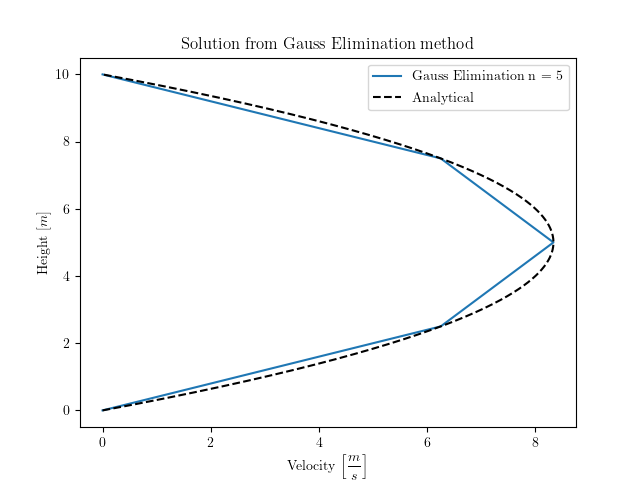
\includegraphics[width=\textwidth]{./code/plot/plot_Gauss Elimination5.png}
	\end{subfigure}
	~
	\begin{subfigure}[b]{0.5\textwidth}
		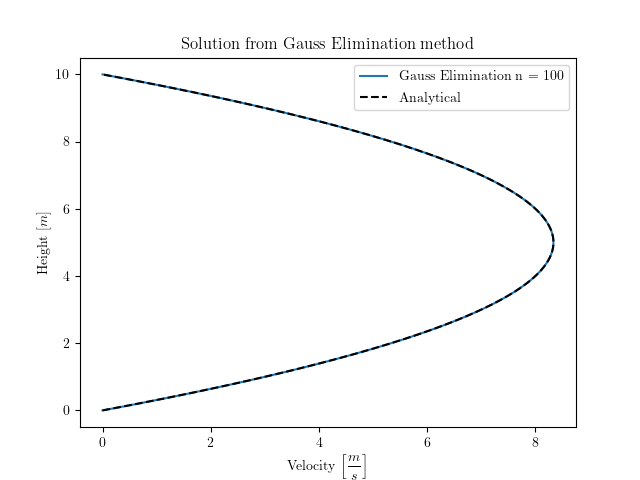
\includegraphics[width=\textwidth]{./code/plot/plot_Gauss Elimination100.png}
	\end{subfigure}
	\caption{Plots using the Gaussian elimination method for $N 	= 5$ and $N = 100$ respectively. The analytical solution is plotted for $N = 1000$ each time.}
	\label{fig:gauss_elim}
\end{figure}
\begin{figure}
	\centering
	\begin{subfigure}[b]{0.5\textwidth}
	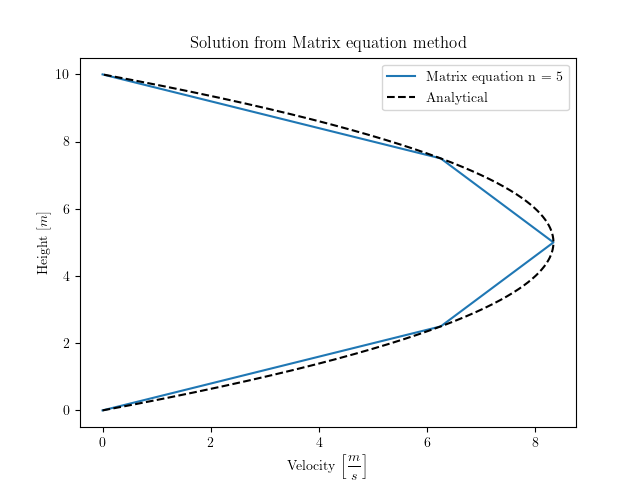
\includegraphics[width=\textwidth]{./code/plot/plot_Matrix equation5.png}
	\end{subfigure}
	~
	\begin{subfigure}[b]{0.5\textwidth}
		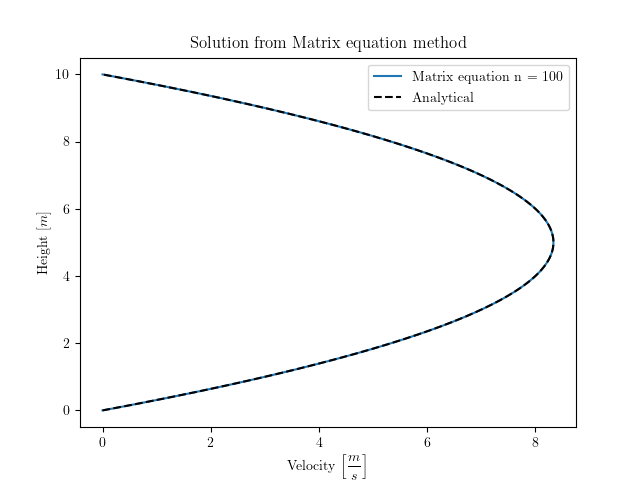
\includegraphics[width=\textwidth]{./code/plot/plot_Matrix equation100.png}
	\end{subfigure}
	\caption{Plots using the Matrix equation method for $N 	= 5$ and $N = 100$ respectively. The analytical solution is plotted for $N = 1000$ each time.}
	\label{fig:matrix_eq}
\end{figure}


\section{Problem 3: More finite differences}
We want to write the FTCS(forward Euler, centered in space) of the following equation 
\begin{equation}
\frac{\partial}{\partial t}\rho = k \frac{\partial^2}{\partial x^2 }\rho
\end{equation}
using $s = kdt/dx^2$.
Using the same principle for finding the taylor expansion as we did in equation \ref{eq:diff_disc} to find the expansion of the second derivative, the RHS of the equation. If we take a look at the left hand side(LHS) we have 
\begin{align}
\frac{\partial \rho}{\partial t} &= \frac{\rho(t+dt) - \rho(t)}{dt} + \mathcal{O}(dt)\\
&= \frac{\rho^{n+1} - \rho^2}{dt}
\end{align}
Using this we can insert into our original expression and we get 
\begin{equation}
\frac{\rho^{n+1}_i - \rho^n_i}{dt} = k \frac{\rho^n_{i+1}- 2\rho^n_{i} + \rho^n_{i-1}}{dx^2}
\end{equation}
Where $i$ references the index of the array and $n$ is the current timestep. Using our definition of $s$ we have 
\begin{equation}
\rho^{n+1}_i= s(\rho^n_{i+1}- 2\rho^n_{i} + \rho^n_{i-1}) +  \rho^n_i 
\end{equation}
\begin{equation}
\rho^{n+1}_i= s\rho^n_{i+1} + (1-2s)\rho^n_{i} + s\rho^n_{i-1} 
\end{equation}
which would be our FTCS. 

We also want to find the iFTCS(implicit Euler, centered in space) version of the same equation. This is straight forward to find. The final expression is our equation looking into the future, and knowing the current value. So the method is the same as for the FTCS, so our equation then becomes 
\begin{equation}
\rho^{n+1}_i + \rho^{n}_i= s\rho^{n+1}_{i+1} -2s\rho^{n+1}_{i} + s\rho^{n+1}_{i-1} 
\end{equation}
Here we have no good way of solving the RHS as we don't know the value of it. We can rearrange the equation to the following 
\begin{equation}
-s\rho^{n+1}_{i+1} +(1+2s)\rho^{n+1}_{i} - s\rho^{n+1}_{i-1}  = \rho^n_i\label{eq:implit}
\end{equation}
We now how 3 unkowns on the LHS. Let us look back at the simpler scheme we had in problem 2. We see that our matrix equation would take the form of $\mathbf{A}\rho^{n+1} = \rho^n + \vec{b}$. We are given that $\rho(1) = 1$ and $\rho(5) = 0$, the matrix equation, ignoring the end points, that follows is 
\begin{equation}
\begin{split}
\mathbf{A}\rho^{n+1} &= \rho^n + \vec{b}\\
\begin{bmatrix}
1+2s & -s & 0\\
-s & 1 +2s & -s\\
0 & -s & 1+2s
\end{bmatrix}
\vec{\rho^{n+1}} &= \rho^n + 
\begin{bmatrix}
s\\
0\\
0
\end{bmatrix}
\end{split}
\end{equation}
Where $\vec{b}$ is found by setting up the set of equations and moving the known terms $\rho(1) = 1$ and $\rho(5) = 0$ inserted for the the values in our implicit scheme \ref{eq:implit}. 

We want to solve this equation for $\rho^{n+1}$, giving us $\rho^{n+1} = \mathbf{A}^{-1}(\rho^n+\vec{b})$. We would need to invert the matrix A, doing so numerically gives us
\lstinputlisting{"./code/problem3.py"}

Our equation for $\rho^{n+1}$ now reads 
\begin{equation}
\rho^{n+1} = \mathbf{A}^{-1}
\begin{pmatrix}
\rho^n_2 + s\\
\rho^n_3\\
\rho^n_4 
\end{pmatrix}
\end{equation}
Where $\mathbf{A}^{-1}$ is the matrix found numerically. 

\section{Code addition}
\lstinputlisting[label=tridiag]{"./code/tridiag.py"}
%%% footnote
% rainforest\footnote{Writing out a general case will also take up more paper
% space}.

%%% Matrix with line through between last elements
% \begin{equation}
% \left[
% \begin{array}{cccc|c}
% 1 & c_1/\beta_1 & 0 & 0 & \tilde{f}_1 \\
% 0 & 1 & c_2/\beta_2 & 0  & \tilde{f}_2 \\
% 0 & 0 & 1 & c_3/\beta_3 & \tilde{f}_3 \\
% 0 & 0 & 0 & 1 & \tilde{f}_4
% \end{array}
% \right] \sim
% \left[
% \begin{array}{cccc|c}
% 1 & c_1/\beta_1 & 0 & 0 & \tilde{f}_1 \\
% 0 & 1 & c_2/\beta_2 & 0  & \tilde{f}_2 \\
% 0 & 0 & 1 & 0 & \tilde{f}_3 -\frac{c_3}{\beta_3}\tilde{f}_4 \\
% 0 & 0 & 0 & 1 & \tilde{f}_4
% \end{array}
% \right]
% \end{equation}

%%% Listing
% \lstinputlisting[language=c++, firstline=146,
% lastline=158]{../problems.cpp}

%%% LU matrix, with diag dots for general case
% \begin{equation}
% A = LU =
% \begin{bmatrix}
% 1 & 0 & 0 & \dots & 0 & 0 \\
% l_{21} & 1 & 0 & \dots & 0 & 0 \\
% l_{31} & l_{32} & 1 & \dots & 0 & 0 \\
%   &\vdots & & \ddots & \vdots  & \\
% l_{n-11} & l_{n-12} & l_{n-13} & \dots & 1 & 0 \\
% l_{n1} & l_{n2} & l_{n3} & \dots & l_{nn-1} & 1
% \end{bmatrix}
% \begin{bmatrix}
% u_{11} & u_{12} & u_{13} & \dots & u_{1n-1} & u_{1n} \\
% 0 & u_{22} & u_{23} & \dots & u_{2n-1} & u_{2n} \\
% 0 & 0 & u_{33} & \dots & u_{3n-1} & u_{3n} \\
%   &\vdots & & \ddots & \vdots  & \\
% 0 & 0 & 0 & \dots & u_{n-1n-1} & u_{n-1n} \\
% 0 & 0 & 0 & \dots & 0 & u_{nn}
% \end{bmatrix}
% \end{equation}

%%% Table
% \begin{table}[h]
% \caption{Elapsed time for increasing $n$}
% \begin{tabular}{lcc}
% \hline
% n & TDMA [s] & LU [s] \\ \hline
% 10 & 0.0000035 & 0.00106083 \\
% 100 & 0.0000116 & 0.0022319 \\
% 1000 & 0.000077892 & 0.0677764 \\
% 10000 & 0.000878769 & 21.9247 \\
% 100000 & 0.00757418 & n/a \\
% 1000000 & 0.08616075 & n/a \\
% 10000000 & 0.76534 & n/a
% \end{tabular}
% \label{tab:solver_times}
% \end{table}

%%% Figure
% \begin{figure}[h]
  % \centering
  % \includegraphics[width=0.9\linewidth]{figures/relerror.png}
  % \caption{Plot of maximum relative error as a function of step size}
  % \label{fig:relerror}
% \end{figure}

%%% Cition and bilbliography%%
% # \emph{Thomas Algorithm} \cite{thomasalgo} How to cite.
% \begin{thebibliography}{10}
  % \bibitem{thomasalgo}{Thomas, L.H. (1949), \emph{Elliptic
        % Problems in Linear Differential Equations over a
        % Network}. Watson Sci. Comput. Lab Report, Columbia University,
      % New York.}
      % \bibitem{morten}{Hjorth-Jensen, M. (2015). \emph{Computational
        % Physics - Lecture Notes 2015}. University of Oslo}
    % \bibitem{golub}{Golub, G.H., van Loan, C.F. (1996). \emph{Matrix
          % Computations} (3rd ed.), Baltimore: John Hopkins.}
% \end{thebibliography}

\end{document}
